\chapter{Tehnologii. Arhitectură. Persistență}\label{technical}

Un scop secundar al acestui proiect este explorarea unor metode moderne pentru dezvoltarea aplicațiilor Android. Menținerea unor reguli și structuri clare în organizarea codului aplicației aduce o serie de beneficii, printre care reducerea numărului de bug-uri și ușurința în menținerea și extinderea aplicației pe termen lung și este crucială pentru succesul proiectelor de dimensiuni medii și mari sau la care lucrează mai multe persoane. Dezavantajul acestora este timpul ce trebuie investit la începutul proiectului și o continuă disciplină și atenție din partea programatorilor.

\section{Alegerea platformei Android}

Decizia de a dezvolta această aplicație pentru platforma Android este susținută de motive atât tehnologice, cât și de oportunitate. Conform StatCounter, în Iulie 2019, sistemul de operare Android deținea 76.08\% cotă de piață la nivel global \cite{StatsWorldwide}, 73.71\% la nivelul Europei \cite{StatsEurope} și 81.3\% la nivelul României \cite{StatsRomania}. Aceste cifre justifică prioritizarea platformei Android în dezvoltarea unei aplicații mobile.

Din punct de vedere tehnologic, opțiunile pentru dezvoltarea unei aplicații mobile în 2019 sunt \emph{Android Nativ}, \emph{iOS Nativ} sau \emph{cross-platform}, folosind una dintre cele câteva soluții populare pentru dezvoltare cross-platform (printre care \emph{React Native}, \emph{Flutter} sau \emph{Native Script}). Nevoile tehnice ale acestei aplicații presupun integrarea unei soluții OCR, iar procesarea să se facă pe dispozitiv. Implementarea unei astfel de soluții într-un framework cross-platform nu este o sarcină trivială datorită lipsei de suport și documentație. Alegând între \emph{Android Nativ} și \emph{iOS Nativ}, dezvoltarea pentru Android se poate face de pe orice sistem de operare major, pe când dezvoltarea pentru iOS necesită sistemul de operare macOs. 

Analizând cele două motive de mai sus, am ales \emph{Android Nativ} ca platformă de dezvoltare datorită popularității sistemului de operare, a stabilității ecosistemului de dezvoltare și a suportului și a documentației extensive disponibile. Pentru o viitoare migrare către \emph{iOS}, framework-ul \emph{Flutter} este considerat ca fiind o soluție viabilă.

\section{Tehnologii utilizate}

Dezvoltarea pe platforma \emph{Android Nativ} oferă acces la întreg ecosistemul \emph{JVM}. Acest lucru a permis utilizarea a mai multor librării care nu au fost dezvoltate special pentru Android. În continuare vor fi prezentate tehnologiile folosite în dezvoltarea aplicației și motivația din spatele lor.

\subsection{Kotlin}

Dezvoltarea aplicațiilor Android nu mai înseamnă doar \emph{Java}. \emph{Kotlin} este un limbaj de programare ce rezolvă multe dintre problemele din Java și care, începând din 2017 este suportat în mod oficial de către \emph{Google} ca limbaj de dezvoltare pentru Android, iar din 2019, considerat limbaj preferat pentru Android. Aceasta înseamnă că noile funcționalități ale SDK-ului Android vor fi dezvoltate și oferite cu prioritate către \emph{Kotlin}.

Principalele caracteristici ale acestui limbaj sunt sistemul de tipuri superior, ce suportă inferența tipurilor, existența tipurilor de date care nu pot fi nule (\emph{null safety}), lipsa excepțiilor \emph{verificate} (\emph{checked exceptions}) și diferențierea clară și ușoară între variabile și constante (prin cuvintele cheie \texttt{var} și \texttt{val}). Codul scris în \emph{Kotlin} este de cele mai multe ori mai scurt, mai concis, mai sigur și mai ușor de înțeles decât cel scris în Java.

\subsection{RxJava}

\emph{Programare reactivă} \cite{ReactiveProgramming} este o paradigmă concentrată în jurul reacționării la modificări în starea unui obiect și a devenit populară în ultimii ani, atât pentru dezvoltarea aplicațiilor grafice, cât și pentru aplicațiile de server care procesează fluxuri de date. Avantajele acesteia sunt facilitarea procesării pe mai multe \emph{thread-uri} și abstractizarea componentelor aplicației (\emph{separation of concerns}).

RxJava implementează o serie de abstractizări ce extind ideea de \emph{Observer}\cite{ObseverPattern} și operatori asupra acestor abstractizări pentru a executa computații asupra valorilor reprezentate. Această aplicație folosește RxJava pentru a reprezenta fiecare operație sau unitate computațională și pentru a orchestra aceste computații pe diferite thread-uri, cu scopul de a nu bloca interfața grafică. De exemplu, surprinderea și extragerea informațiilor dintr-o poză este reprezentată folosind abstractizarea \texttt{Single} și este executată pe un thread secundar, în timp ce thread-ul principal afișează un mesaj și răspunde acțiunilor utilizatorului.

\subsection{Android Architecture Components}

\emph{Architecture Components} este o colecție de librării dezvoltată de Google cu scopul de a oferi uneltele necesare pentru a dezvolta aplicații robuste și testabile. Această aplicație folosește:

\begin{itemize}
\item
  \textbf{ViewModel}: gestionează datele aferente unui ecran sau a unei colecții de ecran într-o manieră care ține cont de ciclul de viață al componentelor vizuale (\emph{Activities}, \emph{Fragments}). Folosite pentru a împărtăși date comune între componente vizuale și pentru a nu pierde datele în timpul schimbării configurației, cum ar fi rotirea ecranului.
\item
  \textbf{LiveData}: expune date către componentele vizuale în mod reactiv. Această librărie se aseamănă cu RxJava, fără complexitatea aferentă. În schimb, este dependentă de ciclul de viață al componentelor vizuale, ceea ce evită problemele de tipul \emph{memory leak}.
\item
  \textbf{DataBinding}: este o metodă prin care datele din \emph{ViewModel} pot fi observate în fișierele de \emph{layout} XML.
\item
  \textbf{Room}: este o librărie ce facilitează accesul la baza de date
  \emph{sqlite} disponibilă pe dispozitiv. Se integrează cu
  \emph{LiveData} și \emph{RxJava} pentru a oferi actualizări datelor interogate.
\item
  \textbf{WorkManager}: programează și execută activități de
  \emph{background} sub anumite constrângeri, care să fie executate într-un mod eficient din punct de vedere al bateriei. Folosit pentru a colecta bonurile în cloud.
\end{itemize}

\subsection{Firebase ML Vision}

Google oferă o serie de servicii de machine learning pentru dezvoltatorii de aplicații prin intermediul \emph{Firebase ML Kit}. Unul dintre aceste servicii este \emph{Firebase ML Vision}, ce conține și un modul OCR. Procesarea se poate face atât local, cât și în cloud pentru o performanță sporită. Opțiunea de procesare în cloud este supusă unor tarife, dar procesarea locală este gratuită și oferă o performanță suficient de bună pentru scopul acestei aplicații. Acest serviciu a fost ales în urma unei comparații ce va fi detaliată într-un capitol ulterior.

\subsection{Firebase Cloud Services}

Firebase este o suită de servicii cloud oferită de Google dezvoltatorilor de aplicații mobile și web. Prin folosirea unor servicii cloud este eliminată complexitatea asociată dezvoltării și întreținerii unui serviciu back-end. Dintre serviciile \emph{Firebase}, această aplicație utilizează:

\begin{itemize}
\item
  \textbf{Firestore}: o bază de date noSql ce stochează documente (obiecte JSON). Este folosită pentru funcționalitatea de colectare a bonurilor;
\item
  \textbf{Cloud Storage}: un sistem de foldere și fișiere. Folosit pentru a stoca imaginile asociate bonurilor și fișierele pentru export;
\item
  \textbf{Cloud Functions}: este un serviciu computațional ce este declanșat de diferite evenimente și rulează un mediu \emph{NodeJS} ce execută un anumit program. Este folosit pentru a arhiva fișierele exportate de aplicație și pentru a trimite o notificare cu link-ul de descărcare.
\end{itemize}

\section{Arhitectura aplicației}

Robert C. Martin definește arhitectura unui sistem software ca fiind forma care i se dă de către cei care îl construiesc. Această formă este dată de diviziunea sistemului în componente, de aranjamentul acestor componente și de modul în care aceste componente comunică între ele. Scopul acestei forme este de a facilita dezvoltarea, lansarea și întreținerea sistemului software \cite{ArchitectureDef}.

Arhitectura dezvoltată pentru această aplicație este inspirată de cea prezentată de Robert C. Martin în cartea \emph{Clean Architecture}, dar simplificată și adaptată pentru acest caz. Figura \ref{fig:arhitectura} prezintă nivelurile conceptuale în care este împărțită aplicația. Primele două niveluri și ultimele două niveluri sunt grupate la nivelul codului după rolul pe care acestea îl îndeplinesc în \emph{domain} și \emph{presentation}.

\begin{figure}[h]
  \centering
  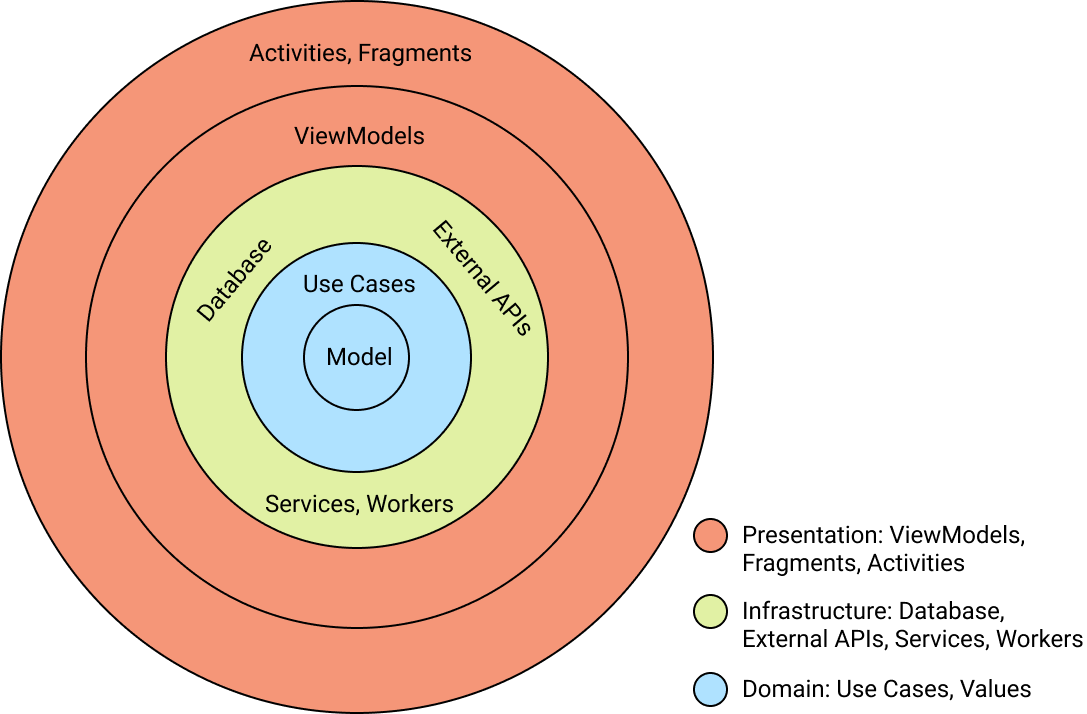
\includegraphics[width=0.465\textwidth]{Architecture.png}
  \caption{Nivelurile conceptuale ale arhitecturii aplicației
  \label{fig:arhitectura}}
\end{figure}

O caracteristică importantă a arhitecturii este aceea că abstractizarea descrește din centru înspre margini. Dependințele în cadrul acesteia sunt orientate către centru. Astfel, un nivel mai abstract nu depinde de un detaliu, ci invers, detaliile depind de abstractizări. Această caracteristică se realizează urmând principiul inversării dependințelor. Pentru a inversa dependințele, un nivel mai înalt definește o interfață care este implementată la un nivel inferior. Această interfață este injectată mai apoi în componenta ce necesită un serviciu implementat la un nivel inferior. Injectarea dependințelor este exemplificată în programul \ref{lst:diExample}.

\lstinputlisting[
  style=javaCodeStyle, 
  caption={ReceiptsUseCaseImpl.kt}, 
  label=lst:diExample
  ]{./code/DiExample.kt}

La nivelul unui \emph{usecase} este necesar accesul la baza de date. Dar la acest nivel detaliul implementării bazei de date nu este relevant. Aceasta poate fi \emph{SQL} sau o simplă colecție în memorie. De aceea este definită interfața \texttt{ReceiptsRepository} care apoi este implementată la nivelul \emph{infrastructure}.

Metoda recomandată pentru injectarea dependințelor în Android este librăria \emph{Dagger 2}. Dacă majoritatea librăriilor pentru injectarea dependințelor utilizează reflexia la \emph{run-time}, Dagger folosește anotările definite în pachetul \texttt{javax.inject} pentru a genera cod la \emph{compile-time}. Avantajul acestei abordări este performanța sporită, dar are dezavantajul necesității de configurare din partea programatorului.

\section{Persistență}

Această aplicație folosește trei medii de persistență pentru stocarea datelor:

\begin{itemize}
\item
  \textbf{sqlite}: datele textuale aferente bonurilor;
\item
  \textbf{internal storage}: imaginile aferente bonurilor;
\item
  \textbf{shared preferences}: datele predefinite și alte configurații;
\end{itemize}

\subsection{SQLITE}\label{sqlite}

Aceasta este o bază de date relațională ce este preinstalată pe sistemul de operare Android. Modelul de date stocat în această bază de date este unul simplu, prezentat în Figura \ref{sqldata}. Aceste tabele sunt generate cu ajutorul librăriei \emph{Room}, folosind codul de mai jos:

\begin{figure}[!ht]
    \centering
    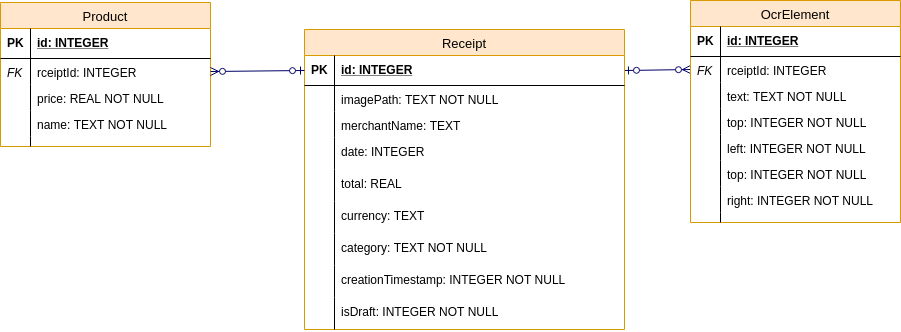
\includegraphics[width=\textwidth]{./figures/ReceiptScanDb.png}
    \caption{Modelul de date SQL \label{sqldata}}
\end{figure}

% \lstinputlisting[style=javaCodeStyle, caption=Entities.kt]{./code/Entities.kt}

\subsection{Spațiul de stocare intern}

Pe spațiul de stocare intern sunt salvate imaginile aferente bonurilor, fiind inaccesibile altor aplicații. Acestea sunt salvate sub un nume aleatoriu, care este salvat în tabela sql (proprietatea imagePath din tabela Receipt).

\subsection{Shared Preferences} \label{technical:sharedPreferences}

\emph{Shared preferences} sunt niște fișiere xml accesibile aplicațiilor Android, unde acestea pot salva valori sub format cheie-valoare. Aici sunt stocate:

\begin{itemize}
    \item
    categoria predefinită pentru bonuri;
    \item
    moneda predefinită;
    \item
    permite sau nu colectarea anonimă a bonurilor;
    \item
    un id unic al aplicației, generat la instalare;
\end{itemize}


